% 
% NIT Patna Resume Template v2.1
% Author: Pavan Kumar Dubasi
% NIT Patna - IMSc., Mathematics (2019-24)
% LinkedIn: https://www.linkedin.com/in/im-pavankumar/
% 

\documentclass[a4paper,11pt]{article}

% Package imports
\usepackage{latexsym}
\usepackage{xcolor}
\usepackage{float}
\usepackage{ragged2e}
\usepackage[empty]{fullpage}
\usepackage{wrapfig}
\usepackage{tabularx}
\usepackage{titlesec}
\usepackage{geometry}
\usepackage{marvosym}
\usepackage{fontawesome5}
\usepackage{verbatim}
\usepackage{enumitem}
\usepackage{fancyhdr}
\usepackage{multicol}
\usepackage{graphicx}
\usepackage{cfr-lm}
\usepackage[T1]{fontenc}
\usepackage{fontawesome5}
\usepackage[hidelinks]{hyperref}
\usepackage{microtype}
\usepackage{array}
\usepackage[most]{tcolorbox}

% Color definitions
\definecolor{darkblue}{RGB}{0,0,139}

% Page layout
\geometry{left=1.4cm, top=0.8cm, right=1.2cm, bottom=1cm}
\setlength{\multicolsep}{0pt} 
\pagestyle{fancy}
\fancyhf{}
\fancyfoot{}
\renewcommand{\headrulewidth}{0pt}
\renewcommand{\footrulewidth}{0pt}
\setlength{\footskip}{4.08pt}

% Hyperlink setup
\hypersetup{
    colorlinks=true,
    linkcolor=darkblue,
    filecolor=darkblue,
    urlcolor=darkblue,
}

% Custom box settings
\tcbset{
    frame code={},
    center title,
    left=0pt,
    right=0pt,
    top=0pt,
    bottom=0pt,
    colback=gray!20,
    colframe=white,
    width=\dimexpr\textwidth\relax,
    enlarge left by=-2mm,
    boxsep=4pt,
    arc=0pt,outer arc=0pt,
}

% URL style
\urlstyle{same}

% Text alignment
\raggedright
\setlength{\tabcolsep}{0in}

% Section formatting
\titleformat{\section}{
  \vspace{-4pt}\scshape\raggedright\large\bfseries
}{}{0em}{}[\color{black}\titlerule \vspace{-7pt}]

% Custom commands
\newcommand{\resumeItem}[2]{
  \item{
    \textbf{#1}{\hspace{0.5mm}#2 \vspace{-0.5mm}}
  }
}

\newcommand{\resumePOR}[3]{
\vspace{0.5mm}\item
    \begin{tabular*}{0.97\textwidth}[t]{l@{\extracolsep{\fill}}r}
        \textbf{#1}\hspace{0.3mm}#2 & \textit{\small{#3}} 
    \end{tabular*}
    \vspace{-2mm}
}

\newcommand{\resumeSubheading}[4]{
\vspace{0.5mm}\item
    \begin{tabular*}{0.98\textwidth}[t]{l@{\extracolsep{\fill}}r}
        \textbf{#1} & \textit{\footnotesize{#4}} \\
        \textit{\footnotesize{#3}} &  \footnotesize{#2}\\
    \end{tabular*}
    \vspace{-2.4mm}
}

\newcommand{\resumeProject}[4]{
\vspace{0.5mm}\item
    \begin{tabular*}{0.98\textwidth}[t]{l@{\extracolsep{\fill}}r}
        \textbf{#1} & \textit{\footnotesize{#3}} \\
        \footnotesize{\textit{#2}} & \footnotesize{#4}
    \end{tabular*}
    \vspace{-2.4mm}
}

\newcommand{\resumeSubItem}[2]{\resumeItem{#1}{#2}\vspace{-4pt}}

% Fixed bullet point definitions
\renewcommand{\labelitemi}{$\vcenter{\hbox{\tiny$\bullet$}}$}
\renewcommand{\labelitemii}{$\vcenter{\hbox{\tiny$\bullet$}}$}

% List commands with proper margins - FIXED ALIGNMENT
\newcommand{\resumeSubHeadingListStart}{\begin{itemize}[leftmargin=*,labelsep=1mm]}
\newcommand{\resumeHeadingSkillStart}{\begin{itemize}[leftmargin=*,itemsep=1.7mm, rightmargin=2ex]}
\newcommand{\resumeItemListStart}{\begin{itemize}[leftmargin=3ex, labelsep=1mm, itemsep=0.5mm, rightmargin=0pt]}

\newcommand{\resumeSubHeadingListEnd}{\end{itemize}\vspace{2mm}}
\newcommand{\resumeHeadingSkillEnd}{\end{itemize}\vspace{-2mm}}
\newcommand{\resumeItemListEnd}{\end{itemize}\vspace{-2mm}}

\newcommand{\cvsection}[1]{%
\vspace{2mm}
\begin{tcolorbox}
    \textbf{\large #1}
\end{tcolorbox}
    \vspace{-4mm}
}

\newcolumntype{L}{>{\raggedright\arraybackslash}X}%
\newcolumntype{R}{>{\raggedleft\arraybackslash}X}%
\newcolumntype{C}{>{\centering\arraybackslash}X}%

% Commands for icon sizing and positioning
\newcommand{\socialicon}[1]{\raisebox{-0.05em}{\resizebox{!}{1em}{#1}}}
\newcommand{\ieeeicon}[1]{\raisebox{-0.3em}{\resizebox{!}{1.3em}{#1}}}

% Font options
\newcommand{\headerfonti}{\fontfamily{phv}\selectfont}
\newcommand{\headerfontii}{\fontfamily{ptm}\selectfont}
\newcommand{\headerfontiii}{\fontfamily{ppl}\selectfont}
\newcommand{\headerfontiv}{\fontfamily{pbk}\selectfont}
\newcommand{\headerfontv}{\fontfamily{pag}\selectfont}
\newcommand{\headerfontvi}{\fontfamily{cmss}\selectfont}
\newcommand{\headerfontvii}{\fontfamily{qhv}\selectfont}
\newcommand{\headerfontviii}{\fontfamily{qpl}\selectfont}
\newcommand{\headerfontix}{\fontfamily{qtm}\selectfont}
\newcommand{\headerfontx}{\fontfamily{bch}\selectfont}

% Define personal information
\newcommand{\name}{Nayini Gowtham Reddy}
\newcommand{\course}{Bachelor of Technology}
\newcommand{\roll}{21951A0554}
\newcommand{\phone}{8374563012}
\newcommand{\emailb}{gowtham5.gr15@gmail.com}
\newcommand{\github}{gowtham-creator}
\newcommand{\website}{https://example.com/}
\newcommand{\linkedin}{GowthamReddy}
\newcommand{\location}[]{}

\begin{document}
\fontfamily{cmr}\selectfont

%----------HEADING-----------------
\parbox{2.35cm}{%
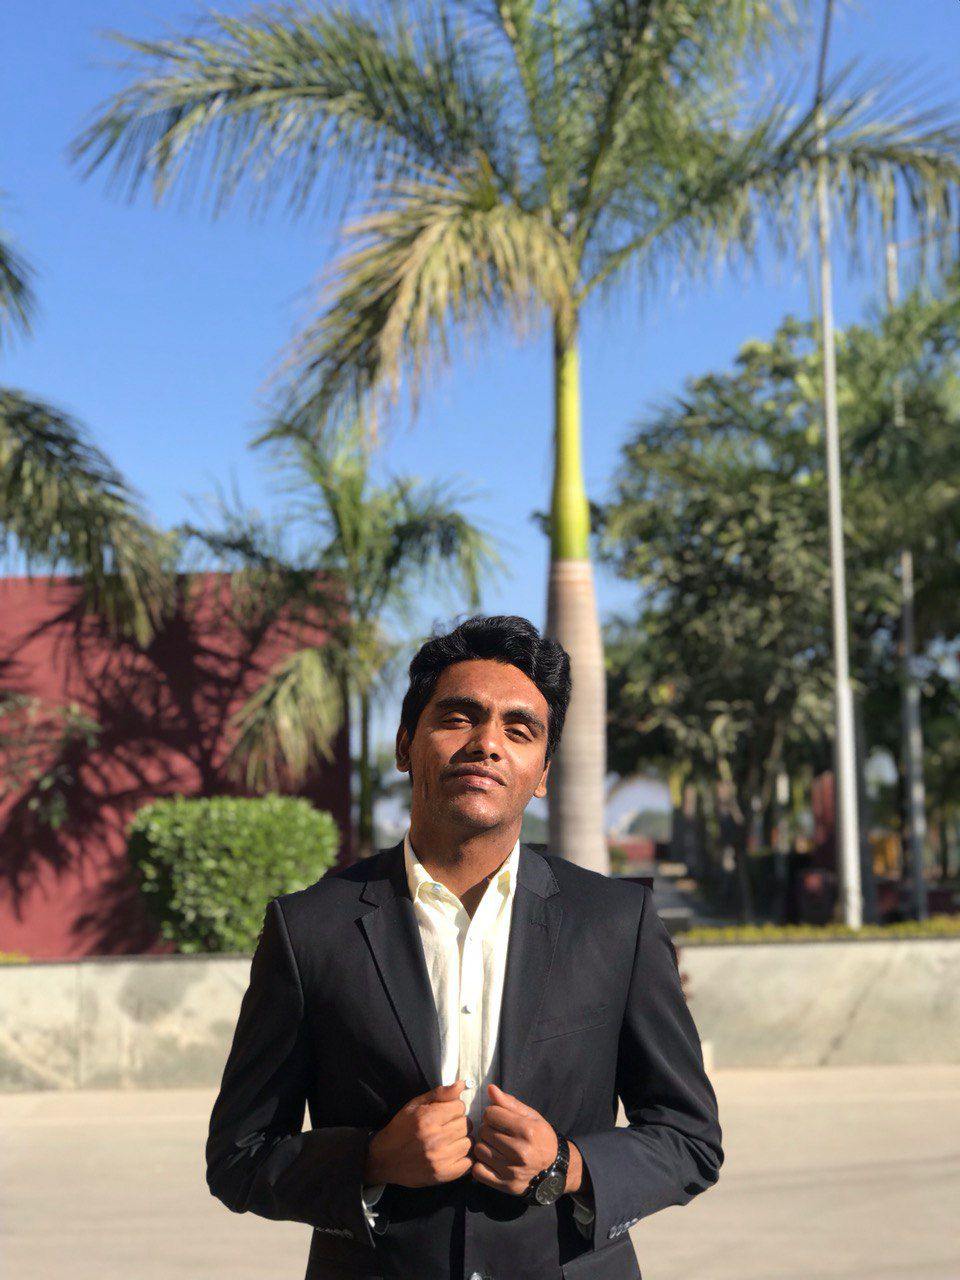
\includegraphics[width=2cm,clip]{gowtham.jpg}
}
\parbox{\dimexpr\linewidth-2.8cm\relax}{
\begin{tabularx}{\linewidth}{L r}
  \textbf{\LARGE \name} & +91-\phone \\
  \course & \href{mailto:\emailb}{\emailb} \\
  Computer Science and Engineering & \href{https://www.linkedin.com/in/gowtham-reddy-821aa41b3/}{linkedin.com/in/\linkedin} \\
  Institute of Aeronautical Engineering, Hyderabad & \href{https://github.com/gowtham-creator}{github.com/\github} \\
\end{tabularx}
}
\vspace{-2mm}

%-----------EDUCATION-----------------
\section{\textbf{Education}}
\vspace{1mm}
\setlength{\tabcolsep}{5pt}
\begin{tabularx}{\textwidth}{|>{\centering\arraybackslash}X|>{\centering\arraybackslash}p{8cm}|>{\centering\arraybackslash}p{3cm}|}
  \hline
  \textbf{Degree/Certificate} & \textbf{Institute/Board} & \textbf{Year} \\
  \hline
  B.Tech, CSE & Institute of Aeronautical Engineering & August, 2025 \\ 
  \hline
  Higher Secondary Education, State Board & Deeksha Junior College & May, 2021 \\
  \hline
  Senior Secondary Education, CBSE Board & Vignan World One School & April, 2019 \\
  \hline
\end{tabularx}
\vspace{-4mm}

%-----------WORK EXPERIENCE-----------------
\section{\textbf{Work Experience}}
\vspace{-0.4mm}
\resumeSubHeadingListStart

\resumeSubheading
{AI Consultant - CUBIXSO \faIcon{briefcase}}{On-Site}
{We Work, RMZ Spire, Hyderabad}{December 2024 - Present}
\resumeItemListStart
\item Developed and deployed \textbf{generative AI} solutions using \textbf{LangChain, LLaMA 3, Qwen and Azure OpenAI} for automation and data intelligence.
\item Built custom \textbf{RAG} pipelines with \textbf{ChromaDB, OCR, Embeddings and vector search} to power enterprise-grade chatbots and document assistants.
\item Collaborated with clients to scope AI use cases, deliver \textbf{proof-of-concepts}, and integrate scalable GenAI systems into production.
\item Contributed to client acquisition by designing high-impact AI demos that translated \textbf{business} needs into \textbf{working AI Solutions and Products.}
\resumeItemListEnd

\resumeSubheading
{Technical Developer Intern - Bolt Abacus \faIcon{briefcase}}{On-Site}
{T-hub Phase-2, Hyderabad}{August 2024 - November 2024}
\resumeItemListStart
\item Developed a dynamic questionnaire feature using \textbf{Node.js} and \textbf{Django} for real-time abacus operations.
\item Leveraged \textbf{data analytics} with \textbf{Generative Models} to build dashboards that analyze student performance metrics and Automate Reports Generation.
\item Created an interactive abacus board using \textbf{Next.js}, \textbf{Node.js}, and \textbf{Flask}, automating report generation Interface post-assignment.
\resumeItemListEnd

\resumeSubheading
{Research and Development Intern - Sria Infotech Pvt Ltd \faIcon{briefcase}}{On-Site}
{T-hub Phase-2, Hyderabad}{June 2023 - June 2024}
\resumeItemListStart
\item Developed a real-time \textbf{Power BI} dashboard, reducing issue resolution times by 30\% with automated screenshot mechanisms. 
\item Automated \textbf{Power BI} User functionality using voice commands through \textbf{Alexa Virtual Assistant} Console Log and \textbf{AWS Lambda}, enhancing client experience by 20\%.
\item Led the development of \textbf{Nxsys}, an AI-powered ticketing tool using \textbf{AutoGen} and \textbf{Crew AI}, increasing automation by 40\%.
\resumeItemListEnd

\resumeSubheading
{Co Founder and CEO - Ava.ai}{Hybrid}
{T-hub Phase-2, Hyderabad}{January 2024 - September 2024}
\resumeItemListStart
\item Developed an AI-powered mental health companion using \textbf{Generative AI}, \textbf{NLP}, and \textbf{Deep learning} for text and audio models.
\item Led a team of 15 engineers and designers, collaborating with technical mentors, researchers, and psychologists for comprehensive product refinement.  
\item Implemented \textbf{agent orchestration}, \textbf{Langflow}, \textbf{Pinecone} for \textbf{vector embeddings}, and \textbf{Neo4j for graph database} integration; managed end-to-end development in \textbf{Flutter} for \textbf{iOS/Android}.
\resumeItemListEnd

\resumeSubheading
{Co Founder and COO - SLiYP}{Remote}
{Hyderabad}{June 2023 - February 2024}
\resumeItemListStart
\item Headed the development of an MVP for a student social media network using \textbf{HTML, CSS, Tailwind, Node.js, React, TypeScript}, and \textbf{Next.js} (MERN).
\item Led a team of 20 developers and engineers, collaborating with VCs for fundraising, and delivering product development. 
\item Developed a mobile application using \textbf{Flutter}, integrated with \textbf{MongoDB}, and deployed on \textbf{AWS}, achieving seamless functionality on the \textbf{Play Store}. 
\resumeItemListEnd

\resumeSubheading
{Associate Software and Machine Learning Developer - Agrodroid}{On-Site}
{IARE, Hyderabad}{November 2022 - May 2023}
\resumeItemListStart
\item Developed an image recognition tool using \textbf{HSV}, \textbf{TensorFlow}, and \textbf{Keras} for cotton \textbf{image classification}, integrated into rover operations.
\item Managed a team of 5 developers, collecting real-time datasets and training \textbf{CNN models} for pre-seeding and cultivation tasks.
\item Led \textbf{data preparation} and \textbf{model development}, improving the rover's \textbf{image recognition} and automation capabilities.
\resumeItemListEnd

\resumeSubheading
{Head of Corporate and Public Relations - E-cell IARE}{On-site}
{IARE, Hyderabad}{June 2023 - October 2023}
\resumeItemListStart
\item Organized large-scale events, promoting entrepreneurship and securing sponsors and Guided startups on funding, legal support, and pitching to investors.
\resumeItemListEnd

\resumeSubHeadingListEnd
\vspace{-6mm}

%-----------PROJECTS-----------------
\section{\textbf{Projects}}
\vspace{-0.4mm}
\resumeSubHeadingListStart

\resumeProject
{Private LAW Gpt and AI Scraping Agent}
{Stream lit, LLaMA 3, OCR, ChromaDB, Advanced RAG}
{May 2025 - June 2025}
{{}\href{https://github.com/your-username/project-b}{\textcolor{darkblue}{}}}
\resumeItemListStart
\item Built a private Legal AI Assistant using \textbf{Langchain, LLaMA 3, and ChromaDB} to automate legal document ingestion, summarization, and Q\&A for Indian law firms.
\item Engineered a full \textbf{Advanced RAG} pipeline with \textbf{OCR}, \textbf{LegalBERT embeddings,} and \textbf{vector search (FAISS)} for citation-backed responses and IPC section detection.
\item Achieved \textbf{90 percent} accuracy in parsing and summarizing scanned court judgments from 30+ Indian legal portals using automated scraping and \textbf{Tesseract OCR}.
\resumeItemListEnd

\resumeProject
{Mulesoft to AWS Conversion}
{Azure OpenAI, AWS IAC, Langchain}
{February 2025 - April 2025}
{}
\resumeItemListStart
\item Developed a Conversion Tool Using \textbf{Langchain} Agent Framework Within StreamLit app to convert Mule code to AWS.
\item \textbf{Lambda functions}, \textbf{AWS IAC} and \textbf{API Gateway configurations} is translated from Mulesoft salesforce code with \textbf{90 percent accuracy} achieved.
\item Implemented in Client System and able to handle \textbf{large Context size} code for translation and System Conversion purpose.
\resumeItemListEnd

\resumeProject
{Blockchain Social Security Service Using Smart Contracts}
{Ethereum, Ganache, Truffle, Solidity}
{August 2024 - March 2025}
{{}\href{https://github.com/your-username/project-a}{\textcolor{darkblue}{}}}
\resumeItemListStart
\item Developed a \textbf{Blockchain}-based social security app with \textbf{Solidity smart contracts} and \textbf{IPFS} for secure data handling.
\item Implemented \textbf{Proof of Stake (PoS)} for \textbf{network security} and automated processes for beneficiary registration and monthly payments.
\item Conducted user testing for validation and \textbf{IEEE Published}.
\resumeItemListEnd

\resumeProject
{DMN Notation and Model Generation with LLMs}
{Stream lit, Llama index, Python, Llama}
{September 2024 - January 2025}
{{}\href{https://github.com/your-username/project-b}{\textcolor{darkblue}{}}}
\resumeItemListStart
\item Developed a tool to generate \textbf{DMN models}, \textbf{Decision Tables} and \textbf{XML} from Business rules document and Excel sheet, achieving \textbf{95 percent validation accuracy} Using \textbf{Llama 2.} 
\item Building a scalable \textbf{full-stack application} to automate \textbf{JSON and Excel} file generation and optimize complex business rules with \textbf{Test Cases}.
\resumeItemListEnd

\resumeProject
{Personalized Power BI automation and navigation tool}
{Power BI, AWS Lambda, REST API's, Alexa Skill Builder}
{September 2023 - July 2024}
{}
\resumeItemListStart
\item Developed a Voice-controlled Power BI tool with \textbf{AWS Lambda} and \textbf{Alexa Console} for navigation, Interaction and Prediction boosting client productivity by \textbf{80 percent}. 
\item Created a Chrome extension with voice and chatbot features using \textbf{Python TTS, Manifest} and \textbf{React.js.} Leveraged \textbf{Rest API's} for \textbf{Analytics} and \textbf{Reporting}.
\resumeItemListEnd

\resumeProject
{Multi Grain Image Processing and Classification}
{Python, Tensorflow, Keras, Scikit-learn}
{June 2024 - August 2024}
{}
\resumeItemListStart
\item Engineered a Grain classification tool with \textbf{90 percent} accuracy on 5,000 images using \textbf{HSV color space} and \textbf{ML models}. \textbf{Python} and \textbf{H5} for Data Handling.
\item Implemented \textbf{TensorFlow} and \textbf{Keras} for \textbf{machine learning}, and LabelImg for accurate \textbf{image annotation} and preparation.
\resumeItemListEnd

\resumeProject
{Resume ATS and Job Recommender AI}
{Nest js, Langchain, Css, Vector Store, AWS S3}
{June 2024 - July 2024}
{}
\resumeItemListStart
\item Built an ATS analysis system achieving \textbf{95 percent accuracy} on 100 Resumes amd 200 Job Postings, providing tailored job recommendations with \textbf{JSON} outputs for Optimal Candidate Matches.
\resumeItemListEnd

\resumeSubHeadingListEnd
\vspace{-8mm}

%-----------SKILLS-----------------
\section{\textbf{Skills}}
\vspace{-0.4mm}
\resumeHeadingSkillStart
\resumeSubItem{Frontend}{: ReactJS, NextJS, CSS, TypeScript}
\resumeSubItem{Backend}{: Node.js, Python, RestAPI}
\resumeSubItem{Databases}{: MongoDB, Firebase, PostgreSQL}
\resumeSubItem{Cloud/DevOps}{: Azure, AWS, Github Actions, Docker, Kubernetes}
\resumeSubItem{AI and LLM}{: Langchain, Langgraph, AI Agents, N8N. MCP, RAG, Azure Open AI, Claude and Gemini API, Multi Agents and Orchestration, Agentic AI, Prompt and Context Engineering, Tensorflow, Sci-kit Learn, Image and Audio Generation}
\resumeSubItem{Data and ML}{: Pandas, Numpy, Matplotlib, Keras, NLP and Model Finetuning}
\resumeSubItem{Soft Skills}{: Leadership, Team Management, Problem Solving, Strategic Thinking, Communication, Collaboration}
\resumeHeadingSkillEnd
\vspace{2mm}

%-----------CERTIFICATIONS-----------------
\section{\textbf{Certifications}}
\vspace{-0.4mm}
\resumeSubHeadingListStart
\resumePOR{}{Generative AI For everyone from \textbf{Coursera}}{}
\resumePOR{}{Generative AI with Large Language Models from \textbf{Coursera}}{}
\resumePOR{}{Improving Deep Neural Networks: Hyperparameter Tuning, Regularization and Optimization from \textbf{Coursera}}{}
\resumePOR{}{Neural Networks and Deep Learning from \textbf{Coursera}}{}
\resumePOR{}{Mathematics For Machine Learning: Linear Algebra from \textbf{Coursera}}{}
\resumePOR{}{Mathematics For Machine Learning: Multivariate Calculus from \textbf{Coursera}}{}
\resumePOR{}{Mathematics for Machine Learning: PCA from \textbf{Coursera}}{}
\resumePOR{}{Machine learning A-Z with AI, python and R from \textbf{Udemy}}{}
\resumePOR{}{Complete machine learning and data science bootcamp from \textbf{Udemy}}{}
\resumePOR{}{AI For Everyone from \textbf{Coursera}}{}
\resumePOR{}{AWS Fundamentals Specialization from \textbf{Coursera}}{}
\resumePOR{}{Microsoft Azure Fundamentals Specialization from \textbf{Coursera}}{}
\resumePOR{}{TEDxIARE Certification of Appreciation from \textbf{TEDx}}{}
\resumeSubHeadingListEnd
\vspace{-6mm}

%-----------ACHIEVEMENTS-----------------
\section{\textbf{Achievements} and \textbf{Awards}}
\vspace{-0.2mm}
\resumeSubHeadingListStart
\resumeItemListStart
\item Selected for Microsoft for Startup Founders \textbf{global} startup program as \textbf{Founder Member}.
\item Chosen for the AWS Build Accelerator, a 10-week \textbf{global} program for \textbf{startup founders}.
\item \textbf{Runner-up} in the AWS Campus Fund \textbf{Startup Pitching} Program.
\item Admitted to the \textbf{MIT Innovation Leadership} Bootcamp, focusing on \textbf{innovation and entrepreneurship}.
\item Shortlisted for \textbf{IIT Hyderabad's} \textbf{Startup Fair} at the \textbf{E-Summit}, showcased SLiYP to investors, Participants and industry leaders.
\item \textbf{Graduated} from Buildspace Season 5, ranking in the top \textbf{7.4 percent} out of 70,000 participants in a rigorous 6-week accelerator program. 
\item Earned \textbf{5-star rating} for Python proficiency in \textbf{Hackerrank.} 
\item \textbf{Ranked} in the \textbf{Top 10 AI startups} out of 10,000 in MATHADEMIA MATH HACK 1.0, 2.0 by T-Hub and the Department of Science and Technology.
\item \textbf{Shortlisted} and selected for Wadhwani's Lift Off Spark Accelerator, a 12-week program for \textbf{scaling startups}.
\item \textbf{Shortlisted} and Selected for \textbf{Google for Startup's} AI Academy, Standing out of thousands of applicants all over India. 
\item \textbf{Merit} in Piano Professional Degree from Trinity College Of London.
\resumeItemListEnd
\resumeSubHeadingListEnd
\vspace{-6mm}

%-----------RESEARCH AND PUBLICATIONS-----------------
\section{\textbf{Research} and \textbf{Publications}}
\vspace{-0.4mm}
\resumeSubHeadingListStart
\resumeSubheading
{Blockchain Enabled Social Security Using Smart Contract}{Sept - 2024}
{Research Paper}{\textbf{Completed}}
\resumeItemListStart
\item Conducted research on implementing Social Security Services using Blockchain technology, Paper submitted to \textbf{2025 Annual International Conference on Data Science, Machine Learning and Blockchain Technology}.
\resumeItemListEnd
\resumeSubHeadingListEnd
\vspace{-5mm}

\end{document}